\chapter[ARQUITETURA PARA PROCESSAMENTO DE DADOS]{ARQUITETURA PARA PROCESSAMENTO DE DADOS}
\label{chapter:architecture}

A \textbf{Arquitetura Kappa} é o padrão de projeto escolhido para servir de
base para a camada de processamento de dados do InterSCity. A Arquitetura
Lambda não justifica a maior complexidade no contexto atual do InterSCity, de
modo que essa escolha facilita a manutenibilidade e adoção da arquitetura pelo
time do InterSCity, só devem aprender uma tecnologia de processamento
\textit{streaming}. A Arquitetura Kappa permitirá a análise em tempo-real sem
que ocorra perda de informações relevantes, o que é importante no contexto de
cidades inteligentes, ao passo em que permite a análise de dados históricos,
desde que estes tenham sido pré-processados. Esta decisão então força a escolha
de uma tecnologia de processamento \textit{streaming}, e um \textit{broker}
adequado.

O \textbf{Apache Spark} é a tecnologia de \textit{streaming} escolhida,
principalmente por dispor nativamente de biblioteca de clusterização e
aprendizagem de máquina. Esta ferramenta ainda facilita, caso necessário, a
troca para a Arquitetura Lambda, por dispor de processamento \textit{batch}.
O \textbf{Apache Kafka} é o \textit{broker} escolhido, sendo esta uma escolha
menos óbvia que a anterior. Embora o RabbitMQ já seja utilizado pelo
InterSCity, e tenha vantagens em certos aspectos em relação ao Kafka, não
dispor de uma interface nativa que o conecte ao Spark ocasionou nessa decisão.
Outro fator importante é o gerenciamento nativo de \textit{log} por parte do
Kafka, que ajuda na implantação da Arquitetura Kappa. É importante também
ressaltar que esta mudança de \textit{broker} ocorrerá somente na arquitetura
de processamentos, não trazendo mudanças aos microserviços do InterSCity.
A Figura \ref{fig:stack} ilustra a pilha de tecnologias que deve compor a
Arquitetura Kappa no InterSCity.

\begin{figure}
  \centering
    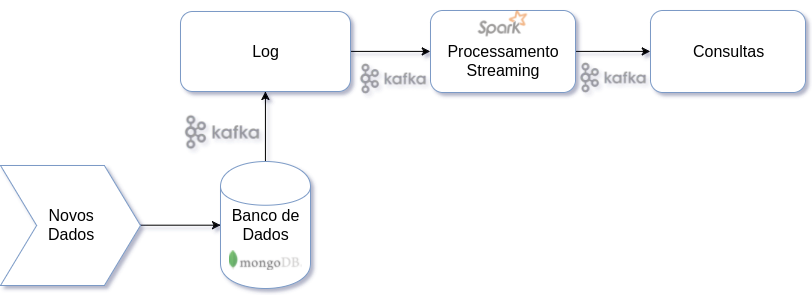
\includegraphics[scale=0.5]{figuras/kappa_tools.png}
  \caption{Pilha de tecnologias utilizadas - Apache Kafka, Apache Spark e MongoDB.}
  \label{fig:stack}
\end{figure}


\section{IMPLEMENTAÇÃO}

